%%%%%%%%%%%%%%%%%%%%%%%%%%%%%%%%%%%%%%%%%%%%%%%%%
%%         Projet Dome geodesique              %%
%%                                             %%
%%   Planète Sciences / InCOGnu / Tetalab      %%
%%%%%%%%%%%%%%%%%%%%%%%%%%%%%%%%%%%%%%%%%%%%%%%%%

%% Authors: Séverin Lemaignan


\documentclass[a4paper,12pt]{report}

\usepackage{fullpage}

\usepackage{graphicx}

\usepackage{xcolor}

\usepackage{ifthen}

\usepackage[utf8]{inputenc}

\usepackage[T1]{fontenc}
\pdfmapfile{+ubuntu-regular.map}
\pdfmapfile{+ubuntu-it.map}
\pdfmapfile{+ubuntu-bold.map}
\renewcommand{\rmdefault}{Ubuntu}

\usepackage{listings}
\usepackage{framed}
\usepackage{wrapfig}
\usepackage{fancyhdr} %headers and footers
\pagestyle{fancy}

\usepackage{url}
\usepackage{hyperref}
\usepackage{sectsty}

\usepackage{enumerate}

\usepackage{pdfpages} %% To add a cover to the doc
\usepackage{booktabs}
\usepackage{rotating}

% Fixme notes
\usepackage[draft,footnote,marginclue]{fixme}


\usepackage[french]{babel}

\graphicspath{{images/}}

%################# En-tête et pieds de page avec fancyhdr
\headheight=14.85pt
%pour récupérer les noms de section en minuscule
\renewcommand{\chaptermark}[1]{\markboth{#1}{}}
\renewcommand{\sectionmark}[1]{\markright{#1}}

\fancyhf{}
\fancyhead[RO,LE]{\bfseries\leftmark}
%\fancyhead[LE]{\rightmark}
\fancyfoot[LE,RO]{\bfseries\thepage}
\renewcommand{\headrulewidth}{0.3pt}
%\addtolength{\headheight}{2pt}
\addtolength{\headsep}{20pt}
\addtolength{\footskip}{10pt}
\renewcommand{\footrulewidth}{0pt}
\fancypagestyle{plain}{\fancyhead{}\renewcommand{\headrulewidth}{0pt}}

%%%%%%%%%%%%%%%%%%%%%%%%%%%%%%%%%%%%%%%%%%%%%%%%%%%%%%%%%%%%%%%%%%%%%%%%%%%%%%%%%
%%%%%%%%%%%%%%%%%%%%%%%%%%%%%%%%%%%%%%%%%%%%%%%%%%%%%%%%%%%%%%%%%%%%%%%%%%%%%%%%%

\title{
	
\includegraphics[width=12cm]{logos.pdf}\\
	\vfill
	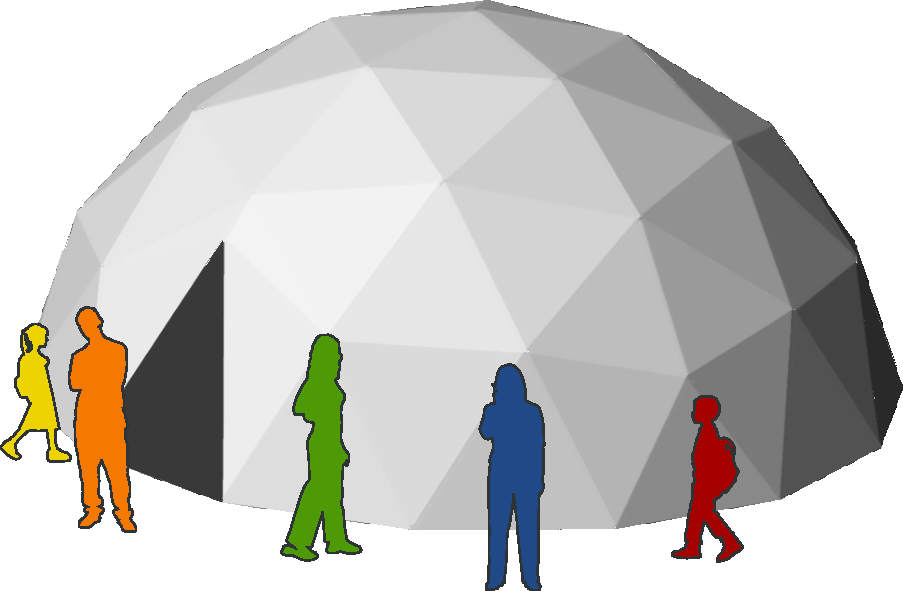
\includegraphics[width=9cm]{general.pdf}\\
	\vspace{3em}
	\LARGE{\textbf{Dôme géodésique}}\\[1cm]
	\large{Projet inter-associatif d'espace d'expérimentation et de projection}\\[1cm]
	\vfill
}

\author{
Séverin Lemaignan
}

%%%%%%%%%%%%%%%%%%%%%%%%%%%%%%%%%%%%%%%%%%%%%%%%%%%%%%%%%%%%%%%%%%%%%%%%%%%%%%%%%
%%%%%%%%%%%%%%%%%%%%%%%%%%%%%%%%%%%%%%%%%%%%%%%%%%%%%%%%%%%%%%%%%%%%%%%%%%%%%%%%%
\begin{document}

\IfFileExists{cover.pdf}{
\includepdf[pages=-, fitpaper]{cover.pdf}
\thispagestyle{empty}
\cleardoublepage
}

\maketitle

\tableofcontents

%%%%%%%%%%%%%%%%%%%%%%%%%%%%%%%%%%%%%%%%%%%%%%%%%%%%%%%%%%%%%%%%%%%%%%%%%%%%%%%%%
%%%%%%%%%%%%%%%%%%%%%%%%%%%%%%%%%%%%%%%%%%%%%%%%%%%%%%%%%%%%%%%%%%%%%%%%%%%%%%%%%

\chapter{Introduction}

Fin 2011 est née l'idée, lors d'une formation organisée à Planète Sciences, de construire un dôme hémisphérique pour réaliser des projections vidéos immersives.


\chapter{Possibilités offertes par le dôme}

Le dôme qu'il est prévu de construire est une structure métallique de 8m de diamètre sur environ 3,2m de haut.

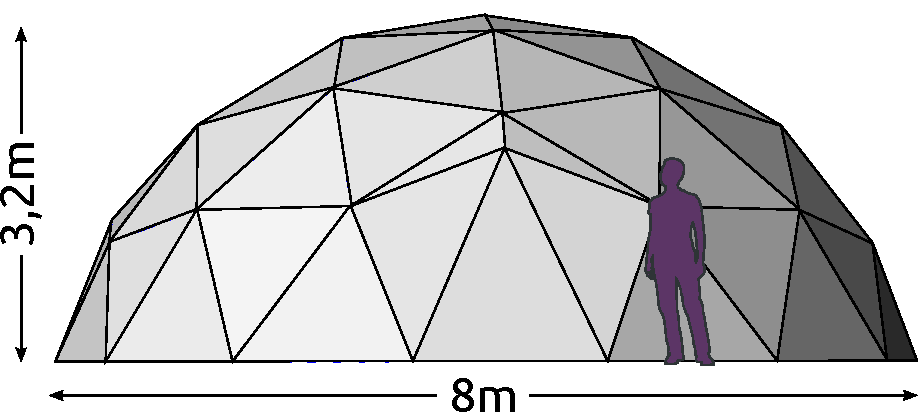
\includegraphics[width=9cm]{dimensions.pdf}

Il permetterait d'accueillir confortablement 25 adultes debout.

Au moins trois types d'activités peuvent y être envisagées:

\begin{itemize}
	\item lors de manifestations associatives publiques, le dôme peut 
	être une zone d'accueil du public, avec un caractère inhabituel et 
	donc attirant. Il peut aussi être un espace remarquable pour des 
	ateliers. De part sa forme et sa taille, il invite aussi à être utilisé comme 
	point central lors de l'installation de manifestations avec de 
	nombreux stands ou tentes.
	\item le dôme sera équipé d'une couverture opaque, bien adaptée à 
	des projections vidéos immersives ``à 360''. C'est l'utilisation 
	originale prévue pour le dôme. L'équipement de projection adéquat 
	(lentille hémisphérique, vidéo-projecteur) fait parti du présent projet.
	De nombreux types de projections sont possible, de films "standards" 
	à des environnements 3D dynamiques et interactifs en passant par des applications
	type planétarium. La section suivant décrit quelques expériences possibles.
	\item enfin, le dôme est aussi envisagé comme une plateforme 
	d'expérimentation inter-associative : c'est un espace atypique, 
	modulable, créé par et pour les bénévoles des trois associations. 
	Nous aimerions qu'il devienne un endroit de création de contenus 
	artistiques et scientifiques (en fonction des spécificités de chaque 
	association) où puissent aussi avoir lieu des rencontres et des échanges
	de savoir-faire. Un espace expérimental ouvert.
\end{itemize}

\chapter{Activités prévues}

\chapter{Description technique}

\chapter{Budget prévisionnel}

%\begin{sidewaystable}
\begin{center}
\begin{tabular}{lrlr}
    \toprule
    Intitulé      & Montant \\
    \midrule
    
    \textbf{Dôme}                         &          \\
    \phantom{ZZ}Tubes acier               &    300   \\
    \phantom{ZZ}Peinture                  &     50   \\
    \phantom{ZZ}Visserie                  &     50   \\
    \phantom{ZZ}Bâche                     &   1500   \\
    \textit{Sous-total dôme}              & \underline{1900} \\
    
    \textbf{Équipement projection}        &           \\
    \phantom{ZZ}Vidéoprojecteur           &    1500   \\
    \phantom{ZZ}Lentille fish-eye         &     150   \\
    \phantom{ZZ}Matériel optique          &     250   \\
    \textit{Sous-total vidéo}             & \underline{1900} \\
    
    \textbf{Outillage}                    &           \\
    \phantom{ZZ}Presse                    &     200   \\
    \phantom{ZZ}Petit outillage (pinceaux...) &  50   \\
    \textit{Sous-total outillage}         & \underline{250} \\
    
    \textbf{Total}                        & \fbox{4050} \\
    \bottomrule                
    \end{tabular}

\end{center}    
%\end{sidewaystable}

\chapter{Annexe : proposition de convention inter-associative}

\IfFileExists{convention.pdf}{
\includepdf[pages=-, frame=true]{convention.pdf}

}

%%%%%%%%%%%%%%%%%%%%%%%%%%%%%%%%%%%%%%%%%%%%%%%%%%%%%%%%%%%%%%%%%%%%%%%%%%%%%%%%%%%%%%%%%%%%%%%%%%%%%%%
\clearpage
\thispagestyle{empty}
~
\vfill
\begin{center}
	L'ensemble de ce projet est diffusé sous license libre Creative Commons Paternité-Partage à l'identique.\\
	\vspace{2cm}
	
\includegraphics[scale=0.5]{logo_cc.png}
\end{center}

\vfill

\begin{center}
	Les sources de ce document peuvent être téléchargées depuis le site GitHub.
	\url{http://github.com/skadge/dome/}
\end{center}

\vfill

\end{document}

